\documentclass[11pt, letterpaper, notitlepage]{article}
\usepackage[utf8]{inputenc}
\usepackage{amsmath}
\usepackage{amsfonts}
\usepackage{amsthm}
\usepackage{mathtools}
\usepackage{setspace}
\usepackage{enumitem}

\renewcommand{\abstractname}{Overview}

\usepackage{color}   %May be necessary if you want to color links
\usepackage{hyperref}
\hypersetup{
    colorlinks,
    citecolor=blue,
    filecolor=blue,
    linkcolor=blue,
    urlcolor=blue
}

\title{Competition Launch Report \\ Dota 2 Message Classification for Auto-Moderation Purposes}
\author{Richard Motorgeanu - motorger - 400436012\\ Jacquelyn Pohl - pohlj - 400455088\\ Nicholas Gyorgypal - gyorgypn - 400446785}
\date{\today}

\DeclarePairedDelimiter\abs{\lvert}{\rvert}%

\DeclarePairedDelimiter\ceil{\lceil}{\rceil}
\DeclarePairedDelimiter\floor{\lfloor}{\rfloor}

\begin{document}
\maketitle


\vspace{12em}

\textbf{Content Warning}: This document deals with the categorization of toxic content and messages found online that contain profane, vulgar, or offensive content. Proceed with caution.

\newpage

\section[1]{Agreement}

We used the Percentage Agreement metric to calculate agreement for our data. We chose this metric as the other 3 that were suggested didn't really apply to our situation or was more difficult to calculate. We didn't have more than 2 annotators, so Fleiss' Kappa wouldn't work. All the duplicated data in our datasets were annotated, so there was no need to consider Krippendorff's Alpha. Finally, since we had 8 categories, computing Cohen's Kappa would result in a lot of probability calculations ($\sim 50$).

Using Percentage Agreement, we got an agreement score of 39\%. 

Since a lot of people mentioned that they struggled to differentiate between the different types of negativity, we also did a separate calculation where we grouped up categories 3, 4, and 5 and considered them equal. With this, we got an agreement score of 45\%.

We did another scenario, where we calculated whether people agreed on if a message was toxic (categories 3, 4, and 5) or not toxic (categories 0, 1, 2, 6, 7). This resulted in an agreement score of 68\%.

Finally, we did one last scenario, where we calculated whether people agreed on if a message was toxic or not toxic, and disregarded instances where one or both annotators labelled a message as non-English. This resulted in an an agreement score of 62\%.

\section[2]{Ground Truth Labels}

For the ground truth, any piece of data that was annotated by only 1 person was determined to be the ground truth (for simplicity).

For duplicate pieces of data, if both annotators agreed, we let that be the ground truth. Otherwise, we did one of two things.

If the data came from data segment 1 and 2, we gave priority to data segment 1 as the annotator 1 has more experience with competitive games like Dota.

For data segment 3 and 4, it seemed like both annotators were inexperienced with competitive gaming and chats, so we had a member of our group go through their labels and pick which was more accurate, and let this act as a tie-breaker.

Below we've also attached the distribution of our categories.

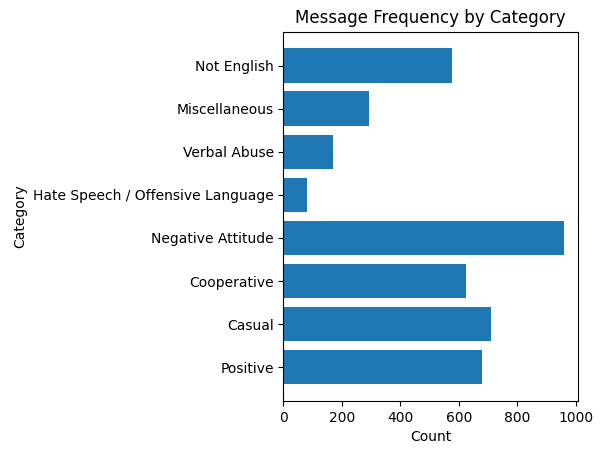
\includegraphics[scale=0.8]{frequency_plot}

\section[3]{Baseline}

\section[4]{Codabench and Google Slides}

\end{document}